%%%%%%%%%%%%%%%%%%%%%%%%%%%%%%%%%%%%%%%%%%%%%%%%%%%%%%%%%%%%%%%%%%%%%%%%%%%%%%%%
% TUM-Vorlage: Plakat A3 Querformat
%%%%%%%%%%%%%%%%%%%%%%%%%%%%%%%%%%%%%%%%%%%%%%%%%%%%%%%%%%%%%%%%%%%%%%%%%%%%%%%%
%
% Rechteinhaber:
%     Technische Universität München
%     https://www.tum.de
% 
% Gestaltung:
%     ediundsepp Gestaltungsgesellschaft, München
%     http://www.ediundsepp.de
% 
% Technische Umsetzung:
%     eWorks GmbH, Frankfurt am Main
%     http://www.eworks.de
%
%%%%%%%%%%%%%%%%%%%%%%%%%%%%%%%%%%%%%%%%%%%%%%%%%%%%%%%%%%%%%%%%%%%%%%%%%%%%%%%%

%%%%%%%%%%%%%%%%%%%%%%%%%%%%%%%%%%%%%%%%%%%%%%%%%%%%%%%%%%%%%%%%%%%%%%%%%%%%%%%%
\documentclass[a3, landscape, plainsections]{sciposter}
\newcommand{\PlakatFormat}{A3 quer}

\documentclass{scrlttr2} % Dokumentenklasse: KOMA-Skript Letter

\usepackage[utf8]{inputenc} % Textkodierung: UTF-8
\usepackage[T1]{fontenc} % Zeichensatzkodierung

\usepackage{calc} % Berechnungen

\usepackage[ngerman]{babel} % Deutsche Lokalisierung
\usepackage{graphicx} % Grafiken
\usepackage[absolute]{textpos} % Positionierung

% Silbentrennung:
\usepackage{hyphenat}
%\tolerance 2414
%\hbadness 2414
%\emergencystretch 1.5em
%\hfuzz 0.3pt
%\widowpenalty=10000     % Hurenkinder
%\clubpenalty=10000      % Schusterjungen
%\vfuzz \hfuzz

% Euro-Symbol:
\usepackage[gen]{eurosym}
\DeclareUnicodeCharacter{20AC}{\euro{}}

% Schriftart Helvetica:
\usepackage[scaled]{helvet}
\renewcommand{\familydefault}{\sfdefault}

\usepackage{mathptmx} % skalierbare Formelschriften

\usepackage{tabto} % Tabulatoren
\usepackage{lastpage} % Letzte Seitenzahl auslesen

\usepackage{tabularx} % flexiblere Tabellen
\usepackage{environ} % flexiblere Definition von Environments

\setlength{\PlakatFusszeileHoehe}{20mm}
\setlength{\PlakatFusszeilePositionUnten}{11.5mm}
\renewcommand{\PlakatFusszeileSpaltenzahl}{5}

\setlength{\PlakatSeiteRand}{18mm}
\setlength{\PlakatKopfzeileHoehe}{24mm}
\setlength{\PlakatKopfzeileAbstand}{10mm}
\setlength{\PlakatKopfzeilePositionUnten}{25.5mm}
\setlength{\PlakatUniversitaetLogoBreite}{34mm}
\setlength{\PlakatFakultaetLogoBreite}{21.5mm}
\setlength{\PlakatPositionLinks}{7.5mm}
\setlength{\PlakatFakultaetslogoPositionKorrekturLinks}{27.3mm}
\setlength{\PlakatFakultaetslogoPositionKorrekturOben}{1.3mm}
\setlength{\PlakatFakultaetslogoAbstandRechts}{6mm}
\setlength{\PlakatUniversitaetslogoPositionKorrekturLinks}{7.5mm}
\setlength{\PlakatSpaltenAbstand}{7mm}
\setlength{\PlakatSchriftNormalGroesse}{16pt}
\setlength{\PlakatSchriftNormalZeilenabstand}{20pt}
\setlength{\PlakatAufzaehlungAbstandLinks}{0.82em}

\newcommand{\PlakatTitelSchriftgroesse}{\fontsize{34}{41}\selectfont}

\newcommand{\PlakatTitelEins}[1]{{\PlakatTitelSchriftgroesse #1}\\[40pt]}
\newcommand{\PlakatTitelZwei}[1]{{\fontsize{25}{30}\selectfont #1}\\[22pt]}
\newcommand{\PlakatTitelDrei}[1]{{\fontsize{20}{24}\selectfont #1}\\[60pt]}

\newcommand{\PlakatKopfzeileSchriftgroesse}{\fontsize{16}{20}}
\newcommand{\PlakatSchriftStandard}{\PlakatSchriftNormalGroesse\selectfont}
\newcommand{\PlakatFusszeileSchrift}{\fontsize{9}{10.8}\selectfont}
\newcommand{\PlakatBildUnterschrift}[1]{{\\[-2mm]\fontsize{10}{12}\selectfont{}#1}}



\setlength{\PlakatSeiteHoehe}{20.5cm} % !!! NICHT ENTFERNEN !!!
%%%%%%%%%%%%%%%%%%%%%%%%%%%%%%%%%%%%%%%%%%%%%%%%%%%%%%%%%%%%%%%%%%%%%%%%%%%%%%%%
% TUM-Vorlage: Personenspezifische Informationen
%%%%%%%%%%%%%%%%%%%%%%%%%%%%%%%%%%%%%%%%%%%%%%%%%%%%%%%%%%%%%%%%%%%%%%%%%%%%%%%%
%
% Rechteinhaber:
%     Technische Universität München
%     https://www.tum.de
% 
% Gestaltung:
%     ediundsepp Gestaltungsgesellschaft, München
%     http://www.ediundsepp.de
% 
% Technische Umsetzung:
%     eWorks GmbH, Frankfurt am Main
%     http://www.eworks.de
%
%%%%%%%%%%%%%%%%%%%%%%%%%%%%%%%%%%%%%%%%%%%%%%%%%%%%%%%%%%%%%%%%%%%%%%%%%%%%%%%%

% Für die Person anpassen:

\newcommand{\PersonTitel}{Dr.~rer.~nat.}
\newcommand{\PersonVorname}{Erika}
\newcommand{\PersonNachname}{Mustermann}
\newcommand{\PersonStadt}{@Ort@}
\newcommand{\PersonAdresse}{%
    @Adresse@\\%
    @Plz@~\PersonStadt%
}
\newcommand{\PersonTelefon}{@Telefon@}
\newcommand{\PersonFax}{@Fax@}
\newcommand{\PersonEmail}{@E-Mail@}
\newcommand{\PersonWebseite}{@Web@}

\newcommand{\FakultaetAnsprechpartner}{@Ansprechpartner@}
% Fakultät:
\newcommand{\FakultaetName}{@Fakultät@}
\newcommand{\LehrstuhlName}{@Lehrstuhlname@}

\newcommand{\EinstellungBankName}{Bayerische Landesbank}
\newcommand{\EinstellungBankIBAN}{DE10700500000000024866}
\newcommand{\EinstellungBankBIC}{BYLADEMM}
\newcommand{\EinstellungSteuernummer}{143/241/80037}
\newcommand{\EinstellungUmsatzsteuerIdentifikationsnummer}{DE811193231}

\hyphenation{} % eigene Silbentrennung                    % !!! DATEI ANPASSEN !!!
%%%%%%%%%%%%%%%%%%%%%%%%%%%%%%%%%%%%%%%%%%%%%%%%%%%%%%%%%%%%%%%%%%%%%%%%%%%%%%%%


\newcommand{\PlakatTitel}{Überschrift 1 läuft über gesamte Papierbreite}


%%%%%%%%%%%%%%%%%%%%%%%%%%%%%%%%%%%%%%%%%%%%%%%%%%%%%%%%%%%%%%%%%%%%%%%%%%%%%%%%
%%%%%%%%%%%%%%%%%%%%%%%%%%%%%%%%%%%%%%%%%%%%%%%%%%%%%%%%%%%%%%%%%%%%%%%%%%%%%%%%
% EINSTELLUNGEN
%%%%%%%%%%%%%%%%%%%%%%%%%%%%%%%%%%%%%%%%%%%%%%%%%%%%%%%%%%%%%%%%%%%%%%%%%%%%%%%%

% Allgemein:
\newcommand{\AllgemeinGestalter}{ediundsepp Gestaltungsgesellschaft}
\newcommand{\AllgemeinErsteller}{eWorks GmbH}

% Universität:
\newcommand{\UniversitaetName}{Technische Universität München}
\newcommand{\UniversitaetAbkuerzung}{TUM}
\newcommand{\UniversitaetWebseite}{www.tum.de}
\newcommand{\UniversitaetLogoBreite}{19mm}
\newcommand{\UniversitaetLogoHoehe}{1cm}

\newcommand{\UniversitaetAdresse}{%
    Arcisstraße~21\\%
    80333~München%
}

\newcommand{\PraesentationSeitenrand}{8.9mm}
\newcommand\crule[3][black]{\textcolor{#1}{\rule{#2}{#3}}}

\newlength\smallerbaselineskip
\setlength{\smallerbaselineskip}{0.8\baselineskip}

    % Blautöne:
\definecolor{TUMBlau}{RGB}{0,101,189} % Pantone 300
\definecolor{TUMBlauDunkel}{RGB}{0,82,147} % Pantone 301
\definecolor{TUMBlauHell}{RGB}{152,198,234} % Pantone 283
\definecolor{TUMBlauMittel}{RGB}{100,160,200} % Pantone 542

    % Hervorhebung:
\definecolor{TUMElfenbein}{RGB}{218,215,203} % Pantone 7527 -Elfenbein
\definecolor{TUMGruen}{RGB}{162,173,0} % Pantone 383 - Grün
\definecolor{TUMOrange}{RGB}{227,114,34} % Pantone 158 - Orange
\definecolor{TUMGrau}{gray}{0.6} % Grau 60%


\setbeamercolor*{alerted text}{fg=TUMOrange}

\newcommand{\PraesentationSetzeTextfarbe}{%
    \color{PraesentationTextfarbe}%
    \setbeamercolor*{frametitle}{fg=PraesentationTextfarbe}%
    \setbeamercolor*{normal text}{fg=PraesentationTextfarbe}%
    \setbeamercolor{itemize/enumerate body}{fg=PraesentationTextfarbe}%
    \setbeamercolor*{itemize item}{fg=PraesentationTextfarbe}%
}

\newcommand{\PraesentationFarbschemaStandard}{%
    \setbeamercolor*{background canvas}{}%
    \definecolor{PraesentationTextfarbe}{rgb}{0,0,0}%
    \PraesentationSetzeTextfarbe%
}

\newcommand{\PraesentationFarbschemaWeissBlau}{%
    \setbeamercolor*{background canvas}{bg=TUMBlauDunkel}%
    \definecolor{PraesentationTextfarbe}{rgb}{1,1,1}%
    \PraesentationSetzeTextfarbe%
}

\newcommand{\PraesentationFarbschemaWeissSchwarz}{%
    \setbeamercolor*{background canvas}{bg=black}%
    \definecolor{PraesentationTextfarbe}{rgb}{1,1,1}%
    \PraesentationSetzeTextfarbe%
}

\newcommand{\PraesentationTitelseiteInhalt}{%
    \begin{textblock*}{\paperwidth}[0,0](0cm,-\PraesentationSeitenrand - 6.5mm + \PraesentationPositionKorrekturOben)%
        \color{PraesentationTextfarbe}%
        \frametitle{\inserttitle}
        \vspace*{49.4mm}%
        \usebeamerfont{author}\selectfont\insertauthor\\%
        \insertinstitute\\%
        \insertdate%
    \end{textblock*}%
}

\newcommand{\PraesentationSeitenkopfInhalt}[1]{%
    %\vspace*{31.7mm}%
    \begin{textblock*}{1.68cm}[1,0](\paperwidth - \PraesentationSeitenrand - \PraesentationSeitenrand, 0cm)%
        \includegraphics[width=1.68cm]{#1}%
    \end{textblock*}%
    \begin{textblock*}{3cm}[1,0](\paperwidth - \PraesentationSeitenrand, -\PraesentationSeitenrand)%
        \hbox{%
            \color{PraesentationTextfarbe}%
            \hbox{\insertframenavigationsymbol}%
            \hbox{\insertsubsectionnavigationsymbol}%
            \hbox{\insertsectionnavigationsymbol}%
        }%
    \end{textblock*}%
}

\newcommand{\PraesentationBildUhrenturm}{%
    \begin{textblock*}{10.82cm}[1,1](\paperwidth - \PraesentationSeitenrand - \PraesentationSeitenrand, \paperheight - 9mm)%
        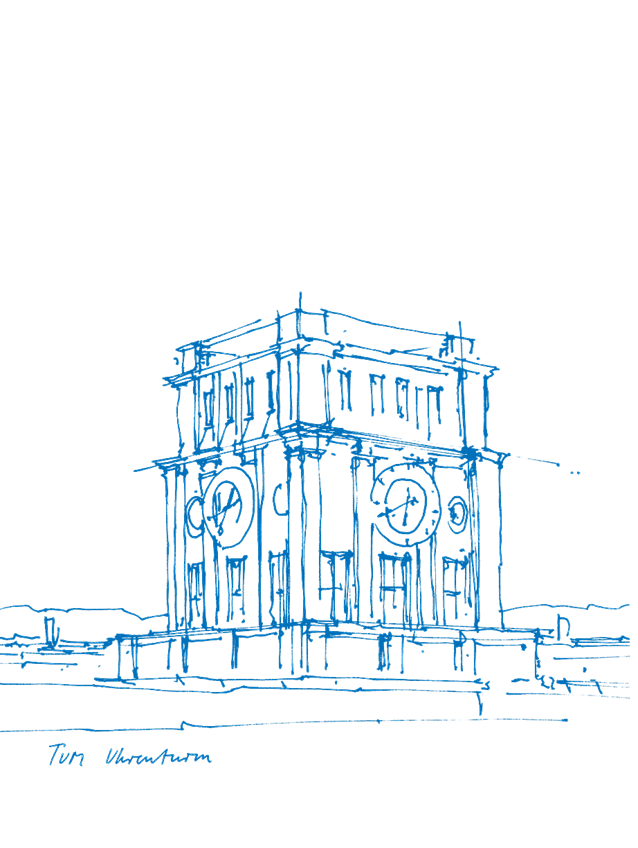
\includegraphics{./Ressourcen/Praesentation/Bilder/TUM_Uhrenturm.png}%
    \end{textblock*}%
}

\newcommand{\PraesentationStartseiteUhrenturm}{%
    \setbeamertemplate{title page}{%
        \PraesentationSeitenkopfInhalt{./Ressourcen/_Bilder/Universitaet_Logo_RGB.pdf}%
        \PraesentationBildUhrenturm%
        \PraesentationTitelseiteInhalt%
    }%
}

\newcommand{\PraesentationStartseiteFlaggen}{%
    \setbeamertemplate{title page}{%
        \begin{textblock*}{\paperwidth}[0,1](-\PraesentationSeitenrand,\paperheight-\PraesentationSeitenrand)%
            
\includegraphics[min width=\paperwidth,max width=\paperheight,min totalsize={\paperwidth}{\paperheight},keepaspectratio,center]{./Ressourcen/Praesentation/Bilder/Universitaet_Flaggen.jpg}%
        \end{textblock*}%
        \PraesentationSeitenkopfInhalt{./Ressourcen/_Bilder/Universitaet_Logo_weiss.pdf}%
        \PraesentationTitelseiteInhalt%
    }%
}

\newcommand{\PraesentationStartseiteLeer}{%
    \setbeamertemplate{title page}{%
        \PraesentationSeitenkopfInhalt{./Ressourcen/_Bilder/Universitaet_Logo_weiss.pdf}%
        \PraesentationTitelseiteInhalt%
    }%
}


\newcommand{\PraesentationMasterStandard}{%
    \PraesentationFarbschemaStandard%
    \PraesentationStartseiteUhrenturm%
    \setbeamertemplate{headline}{%
        \PraesentationSeitenkopfInhalt{./Ressourcen/_Bilder/Universitaet_Logo_RGB.pdf}%
    }%
}

\newcommand{\PraesentationMasterWeissBlau}{%
    \PraesentationFarbschemaWeissBlau%
    \PraesentationStartseiteLeer%
    \setbeamertemplate{headline}{%
        \PraesentationSeitenkopfInhalt{./Ressourcen/_Bilder/Universitaet_Logo_weiss.pdf}%
    }%
}


\newcommand{\PraesentationMasterKopfzeileDreizeiler}{%
    \PraesentationFarbschemaStandard%
    \setbeamertemplate{title page}{%
        \begin{textblock*}{\paperwidth}[0,0](0cm, -7.8mm)%
            \color{TUMBlau}\PraesentationSchriftgroesseDreizeiler\selectfont%
            \LehrstuhlName\\%
            \FakultaetName\\%
            \UniversitaetName\vskip0pt%
            \normalcolor\normalsize\selectfont%
        \end{textblock*}%
        \PraesentationSeitenkopfInhalt{./Ressourcen/_Bilder/Universitaet_Logo_RGB.pdf}%
        \PraesentationBildUhrenturm%
        \PraesentationTitelseiteInhalt%
    }%
    \setbeamertemplate{headline}{%
        \begin{textblock*}{\paperwidth}[0,0](0cm, 0cm)%
            \begin{minipage}[t][2cm][t]{\paperwidth}%
                \color{TUMBlau}\PraesentationSchriftgroesseDreizeiler\selectfont%
                \LehrstuhlName\\[1.38mm]%
                \FakultaetName\\[1.44mm]%
                \UniversitaetName\vskip0pt%
                \normalcolor\normalsize\selectfont%
            \end{minipage}%
        \end{textblock*}%
        \PraesentationSeitenkopfInhalt{./Ressourcen/_Bilder/Universitaet_Logo_RGB.pdf}%
    }%
}

\newcommand{\PraesentationMasterWeissSchwarz}{%
    \PraesentationFarbschemaWeissSchwarz%
    \setbeamertemplate{title page}{%
        \PraesentationTitelseiteInhalt%
        \PraesentationSeitenkopfInhalt{./Ressourcen/_Bilder/Universitaet_Logo_weiss.pdf}%
    }
    \setbeamertemplate{headline}{%
        \PraesentationSeitenkopfInhalt{./Ressourcen/_Bilder/Universitaet_Logo_weiss.pdf}%
    }
}

\newcommand{\PraesentationTitelseite}{\frame[plain]{\titlepage}}
\newcommand{\PraesentationUeberschriftZweizeilig}[2]{\frametitle{#1\\[8mm]#2}}

\setbeamersize{
    text margin left=\PraesentationSeitenrand,
    text margin right=\PraesentationSeitenrand
}

\setbeamertemplate{frametitle}{%
    {\rule{0pt}{42mm + \PraesentationPositionKorrekturOben}\PraesentationSchriftgroesseSehrGross\selectfont\insertframetitle\newline\vspace*{-6.7mm}}%
}

% Aufzählungen:
\newcommand{\PraesentationAufzaehlungEbeneEinsSymbol}{\raise2pt\hbox{\donotcoloroutermaths\usebeamercolor{itemize subitem}\PraesentationSchriftgroesseAufzaehlungszeichen$\bullet$}}
\newcommand{\PraesentationAufzaehlungEbeneZweiSymbol}{\raise1.25pt\hbox{\donotcoloroutermaths\usebeamercolor{itemize subitem}$-$}}
\setbeamertemplate{itemize items}[circle]
\setbeamertemplate{itemize subitem}[triangle]
\setbeamercolor{itemize subitem}{fg=black}
\setbeamerfont{itemize/enumerate subbody}{size=\normalsize}
\setbeamertemplate{itemize item}{\PraesentationAufzaehlungEbeneEinsSymbol}
\setbeamertemplate{itemize subitem}{\PraesentationAufzaehlungEbeneZweiSymbol{}}
%\addtolength{\leftmarginii}{16mm-2pt}%

\newenvironment{PraesentationAufzaehlung}
{%
    \vspace{-\baselineskip}%
    \begin{itemize}%
        \setlength{\itemsep}{0pt}%
        \setlength{\parskip}{0pt}%
        \setlength{\parsep}{0pt}%
        \addtolength{\itemindent}{-1ex}%
}{%
    \end{itemize}%
}

%%%%%%%%%%%%%%%%%%%%%%%%%%%%%%%%%%%%%%%%%%%%%%%%%%%%%%%%%%%%%%%%%%%%%%%%%%%%%%%%
% DOKUMENT
%%%%%%%%%%%%%%%%%%%%%%%%%%%%%%%%%%%%%%%%%%%%%%%%%%%%%%%%%%%%%%%%%%%%%%%%%%%%%%%%


% PDF-Einstellungen:
\hypersetup{
    pdfstartview={Fit},
    pdfproducer={\AllgemeinErsteller},
    pdfcreator={\AllgemeinGestalter}
}

\textblockorigin{\PraesentationSeitenrand}{\PraesentationSeitenrand} % Ursprung für Positionierung

\setbeamerfont{footnote}{size=\PraesentationSchriftgroesseKlein}

\setbeamertemplate{footline}{
    \hbox{%
        \usebeamerfont{footnote}%
        \begin{beamercolorbox}[wd=.9\paperwidth]{}%
            \hspace*{\PraesentationSeitenrand}%
            \PersonTitel{} \PersonVorname~\PersonNachname~(\UniversitaetAbkuerzung) \PraesentationFusszeileZusatz{}%
        \end{beamercolorbox}%
        \begin{beamercolorbox}[wd=.1\paperwidth]{}%
            \insertframenumber{}%
            \raggedleft
            \hspace*{\PraesentationSeitenrand}%
        \end{beamercolorbox}%
        \vspace*{3.25mm}%
    }%
}

\setbeamertemplate{navigation symbols}{}

\begin{document}
\setlength{\baselineskip}{\PraesentationAbstandAbsatz}
\setlength{\parskip}{\baselineskip}
 % !!! NICHT ENTFERNEN !!!
%%%%%%%%%%%%%%%%%%%%%%%%%%%%%%%%%%%%%%%%%%%%%%%%%%%%%%%%%%%%%%%%%%%%%%%%%%%%%%%%

%%%%%%%%%%%%%%%%%%%%%%
%% 2-Spalten-Layout %%
%%%%%%%%%%%%%%%%%%%%%%

\PlakatKopfzeileLeer
\PlakatFusszeile{%
    \textbf{\UniversitaetName}\\
    \FakultaetName\\
    \LehrstuhlName%
}

\PlakatTitelEins{\PlakatTitel}
\PlakatTitelZwei{Überschrift 2 läuft über gesamte Papierbreite}
\PlakatTitelDrei{Überschrift 3 läuft über gesamte Papierbreite oder gemäß Spaltenbreite}

\begin{multicols*}{2}

\renewcommand{\PlakatBeschreibungKurz}{true}
\PlakatUeberschrift{Schriftgröße 11 pt}

Dies ist die Vorlage für das Plakat (DIN \PlakatFormat{}) der Technischen
Universität München (TUM). Sie entspricht dem Corporate Design der TUM und ist für das Betriebssystem Windows getestet und mit TeX Live 2015 kompatibel.

Bitte geben Sie Ihren individuellen Text an den vorgesehenen Stellen ein. Nutzerhinweise finden Sie außerdem in der Liesmich.txt.

\ifx\PlakatBeschreibungKopfzeileUndAbsender\TRUE
\PlakatUeberschrift{Kopfzeile und Absender}

Es stehen mehrere Varianten zur Auswahl. Diese finden Sie auf den nächsten Seiten als Beispiel oder unter \href{http://\UniversitaetWebseite/cd}{\UniversitaetWebseite/cd}, welche für die verschiedenen Nutzergruppen vorgesehen sind.

\fi

\PlakatUeberschrift{Text}

Strukturieren Sie Ihr Plakat möglichst klar und beschränken Sie sich auf die wichtigsten Informationen. Entscheiden Sie sich für einen ein- oder mehrspaltigen Aufbau, linksbündig oder im Blocksatz. Und wählen Sie bei wenig Text eine entsprechend größere Schrift.

\PlakatUeberschrift{Bilder}

\ifx\PlakatBeschreibungKurz\TRUE % BEGINN kurze/lange Beschreibung

Auch wenn Sie Bilder integrieren möchten, können Sie innerhalb des vorgegebenen Rahmens variieren:

\begin{itemize}
\item Das Bild ist an die Breite der Textspalte angepasst
\item Das Bild geht über alle Textspalten
\item Das Bild ist seitenfüllend innerhalb des vorgesehenen Textrahmens (mit weißem Rand)
\item Das Bild ist seitenfüllend bis an den Papierrand (randabfallend) an mindestens drei Seiten
\end{itemize}

Bilder sollten immer eine Bildunterschrift tragen, die ggf. Informationen zum Bild und zur Autorenschaft enthält.
Das Bild sollte immer genügend Abstand zum Text haben. Gleiches gilt für Grafiken.

\else

Auch wenn Sie Bilder integrieren möchten, können Sie innerhalb des vorgegebenen Rahmens variieren:

\begin{itemize}
\item Das Bild ist an die Breite der Textspalte angepasst
\item Das Bild geht über alle Textspalten
\item Das Bild ist seitenfüllend innerhalb des vorgesehenen Textrahmens (mit weißem Rand)
\item Das Bild ist seitenfüllend bis an den Papierrand (randabfallend) an mindestens drei Seiten
\end{itemize}

Bilder sollten immer eine Bildunterschrift tragen, die ggf. Informationen zum Bild und zur Autorenschaft enthält. 
Das Bild sollte immer genügend Abstand zum Text haben. Gleiches gilt für Grafiken.

\ifx\PlakatBeschreibungBeispielbild\TRUE
\PlakatBild[0cm \PlakatBeschreibungBeispielbildBeschnitt{} 0cm 0cm]{./Ressourcen/_Bilder/Sternenhimmel.jpg}{Bildunterschrift, Autor etc}
\fi

\ifx\PlakatBeschreibungDruck\TRUE
\PlakatUeberschrift{Druck}

Achten Sie darauf, dass das Dokument in Originalgröße gedruckt wird, also keine Anpassung an die Druckränder bei Ihren Druckereinstellungen aktiviert ist.
Wählen Sie bitte unbedingt weiße Papiere statt Naturpapier mit starker Braun- oder Graufärbung. Denn nur sie entsprechen dem Charakter des Corporate Designs der TUM. Denken Sie daran, dass auch Papierstärke (Dicke) und Haptik einen Einfluss auf das Druckergebnis haben.
\fi

\fi % ENDE kurze/lange Beschreibung

Weitere Informationen zum Corporate Design der TUM finden Sie unter
\href{http://\UniversitaetWebseite/cd}{\UniversitaetWebseite/cd}


\end{multicols*}

\clearpage


%%%%%%%%%%%%%%%%%%%%%%
%% 3-Spalten-Layout %%
%%%%%%%%%%%%%%%%%%%%%%

\PlakatKopfzeileMitDreizeiler
\PlakatFusszeileLeer

\PlakatTitelEins{\PlakatTitel}
\PlakatTitelZwei{Überschrift 2 läuft über gesamte Papierbreite}
\PlakatTitelDrei{Überschrift 3 läuft über gesamte Papierbreite oder gemäß Spaltenbreite}

\begin{multicols*}{3}

\renewcommand{\PlakatBeschreibungKopfzeileUndAbsender}{false}
\renewcommand{\PlakatBeschreibungKurz}{false}
\renewcommand{\PlakatBeschreibungDruck}{false}
\setlength{\PlakatBeschreibungBeispielbildBeschnitt}{50cm} % Anpassen der Größe des Beispielbildes
\PlakatUeberschrift{Schriftgröße 11 pt}

Dies ist die Vorlage für das Plakat (DIN \PlakatFormat{}) der Technischen
Universität München (TUM). Sie entspricht dem Corporate Design der TUM und ist für das Betriebssystem Windows getestet und mit TeX Live 2015 kompatibel.

Bitte geben Sie Ihren individuellen Text an den vorgesehenen Stellen ein. Nutzerhinweise finden Sie außerdem in der Liesmich.txt.

\ifx\PlakatBeschreibungKopfzeileUndAbsender\TRUE
\PlakatUeberschrift{Kopfzeile und Absender}

Es stehen mehrere Varianten zur Auswahl. Diese finden Sie auf den nächsten Seiten als Beispiel oder unter \href{http://\UniversitaetWebseite/cd}{\UniversitaetWebseite/cd}, welche für die verschiedenen Nutzergruppen vorgesehen sind.

\fi

\PlakatUeberschrift{Text}

Strukturieren Sie Ihr Plakat möglichst klar und beschränken Sie sich auf die wichtigsten Informationen. Entscheiden Sie sich für einen ein- oder mehrspaltigen Aufbau, linksbündig oder im Blocksatz. Und wählen Sie bei wenig Text eine entsprechend größere Schrift.

\PlakatUeberschrift{Bilder}

\ifx\PlakatBeschreibungKurz\TRUE % BEGINN kurze/lange Beschreibung

Auch wenn Sie Bilder integrieren möchten, können Sie innerhalb des vorgegebenen Rahmens variieren:

\begin{itemize}
\item Das Bild ist an die Breite der Textspalte angepasst
\item Das Bild geht über alle Textspalten
\item Das Bild ist seitenfüllend innerhalb des vorgesehenen Textrahmens (mit weißem Rand)
\item Das Bild ist seitenfüllend bis an den Papierrand (randabfallend) an mindestens drei Seiten
\end{itemize}

Bilder sollten immer eine Bildunterschrift tragen, die ggf. Informationen zum Bild und zur Autorenschaft enthält.
Das Bild sollte immer genügend Abstand zum Text haben. Gleiches gilt für Grafiken.

\else

Auch wenn Sie Bilder integrieren möchten, können Sie innerhalb des vorgegebenen Rahmens variieren:

\begin{itemize}
\item Das Bild ist an die Breite der Textspalte angepasst
\item Das Bild geht über alle Textspalten
\item Das Bild ist seitenfüllend innerhalb des vorgesehenen Textrahmens (mit weißem Rand)
\item Das Bild ist seitenfüllend bis an den Papierrand (randabfallend) an mindestens drei Seiten
\end{itemize}

Bilder sollten immer eine Bildunterschrift tragen, die ggf. Informationen zum Bild und zur Autorenschaft enthält. 
Das Bild sollte immer genügend Abstand zum Text haben. Gleiches gilt für Grafiken.

\ifx\PlakatBeschreibungBeispielbild\TRUE
\PlakatBild[0cm \PlakatBeschreibungBeispielbildBeschnitt{} 0cm 0cm]{./Ressourcen/_Bilder/Sternenhimmel.jpg}{Bildunterschrift, Autor etc}
\fi

\ifx\PlakatBeschreibungDruck\TRUE
\PlakatUeberschrift{Druck}

Achten Sie darauf, dass das Dokument in Originalgröße gedruckt wird, also keine Anpassung an die Druckränder bei Ihren Druckereinstellungen aktiviert ist.
Wählen Sie bitte unbedingt weiße Papiere statt Naturpapier mit starker Braun- oder Graufärbung. Denn nur sie entsprechen dem Charakter des Corporate Designs der TUM. Denken Sie daran, dass auch Papierstärke (Dicke) und Haptik einen Einfluss auf das Druckergebnis haben.
\fi

\fi % ENDE kurze/lange Beschreibung

Weitere Informationen zum Corporate Design der TUM finden Sie unter
\href{http://\UniversitaetWebseite/cd}{\UniversitaetWebseite/cd}


\end{multicols*}

\clearpage


%%%%%%%%%%%%%%%%%%%%%%
%% Bild-Layout %%
%%%%%%%%%%%%%%%%%%%%%%

\PlakatKopfzeileMitEinzeiler
\PlakatFusszeileMehrspaltig{
    Hier kann ein längerer Text stehen, der in mehreren Spalten angeordnet wird.
    \vfill\columnbreak
    Durch \texttt{\textbackslash{}vfill\textbackslash{}columnbreak} lässt sich ein Spaltenwechsel erzwingen.
    \vfill\columnbreak~
    \vfill\columnbreak~
}

\PlakatTitelEins{\PlakatTitel}
\PlakatTitelZwei{Überschrift 2 läuft über gesamte Papierbreite}

\PlakatBildGanzseitig[0cm 23cm 0cm 0cm]{./Ressourcen/_Bilder/SternenhimmelQuer.jpg}{Bildunterschrift, Autor etc}

\clearpage


%%%%%%%%%%%%%%%%%%%%%%%%%%%
%% Layout für wenig Text %%
%%%%%%%%%%%%%%%%%%%%%%%%%%%

\PlakatKopfzeileMitEinzeiler
\PlakatFusszeileLeer

\PlakatTitelSchriftgroesse

Wählen Sie für Plakate mit wenig Text gerne eine größere Schrift (siehe Auswahl für Überschriften). Achten Sie bitte darauf, dass die Schriftgröße Zweck und Gebrauch des Plakats entspricht.


%%%%%%%%%%%%%%%%%%%%%%%%%%%%%%%%%%%%%%%%%%%%%%%%%%%%%%%%%%%%%%%%%%%%%%%%%%%%%%%%
\end{document} % !!! NICHT ENTFERNEN !!!
%%%%%%%%%%%%%%%%%%%%%%%%%%%%%%%%%%%%%%%%%%%%%%%%%%%%%%%%%%%%%%%%%%%%%%%%%%%%%%%%
